\documentclass[journal]{IEEEtran}

\ifCLASSINFOpdf
\else
   \usepackage[dvips]{graphicx}
\fi
\usepackage{url}

\hyphenation{op-tical net-works semi-conduc-tor}

\usepackage{graphicx}

% added by zhbli
\usepackage{booktabs}
\usepackage{multirow}
\usepackage{xcolor}  % 图表有颜色
\usepackage{textcomp}
\usepackage{algorithmic}
\usepackage{amsmath}
\usepackage{amssymb}  % 公式分行

\begin{document}

\title{Use Adversarial Template For Model Adaptation For Siamese Networks For Real-Time Visual Object Tracking}

\author{Zhenbang Li, Qiang Wang, Jin Gao, Bing Li, Weiming Hu
\thanks{This paragraph of the first footnote will contain the date on which you submitted your paper for review. It will also contain support information, including sponsor and financial support acknowledgment. For example, This work is supported by the national key R\&D program of china (No. 2018AAA0102802, No. 2018AAA0102803, No. 2018AAA0102800), the NSFC-general technology collaborative Fund for basic research (Grant No. U1636218), the Natural Science Foundation of China (Grant No. 61751212, 61721004, 61972394), Beijing Natural Science Foundation (Grant No. L172051), the Key Research Program of Frontier Sciences, CAS, Grant No. QYZDJ-SSW-JSC040, and the National Natural Science Foundation of Guangdong (No. 2018B030311046).}
\thanks{The next few paragraphs should contain the authors' current affiliations, including current address and e-mail. For example, F. A. Author is with the National Institute of Standards and Technology, Boulder, CO 80305 USA (e-mail: author@boulder.nist.gov).}
\thanks{S. B. Author, Jr., was with Rice University, Houston, TX 77005 USA. He is now with the Department of Physics, Colorado State University, Fort Collins, CO 80523 USA (e-mail: author@lamar.colostate.edu).}}

\markboth{Journal of \LaTeX\ Class Files, Vol. 14, No. 8, August 2015}
{Shell \MakeLowercase{\textit{et al.}}: Bare Demo of IEEEtran.cls for IEEE Journals}
\maketitle

\begin{abstract}
Model update is import for siamese tracker. However, they often modify the offline learned features, break the generalization ability, easy to overfitting. In this paper, we propose a new method to do model adaptation using first frame gt, 
We show that the basic adversarial examples alone can be used to tackle the online update task in object tracking. [4]
Our method involves performing a simple input manipulation: maximizing predicted class scores with gradient descent. Our approach is thus simple to implement, while also requiring minimal tuning. [4]
We propose a novel framework for real-time object tracking with efficient model adaptation. Given an object tracker, our framework learns to fine-tune its input template in only a few gradient-descent iterations using the target ground-truth at the first frame. [3]
To our knowledge, this work is the first attempt to exploit adversarial information for template update in siamese-based trackers. Extensive experiments on recent benchmarks demonstrate that our method achieves better performance than other state-of-the-art trackers.
\end{abstract}


\begin{IEEEkeywords}
Adversarial examples, siamese networks, visual tracking.
\end{IEEEkeywords}


\IEEEpeerreviewmaketitle


\section{Introduction}

\begin{figure}[t]
    \centering
    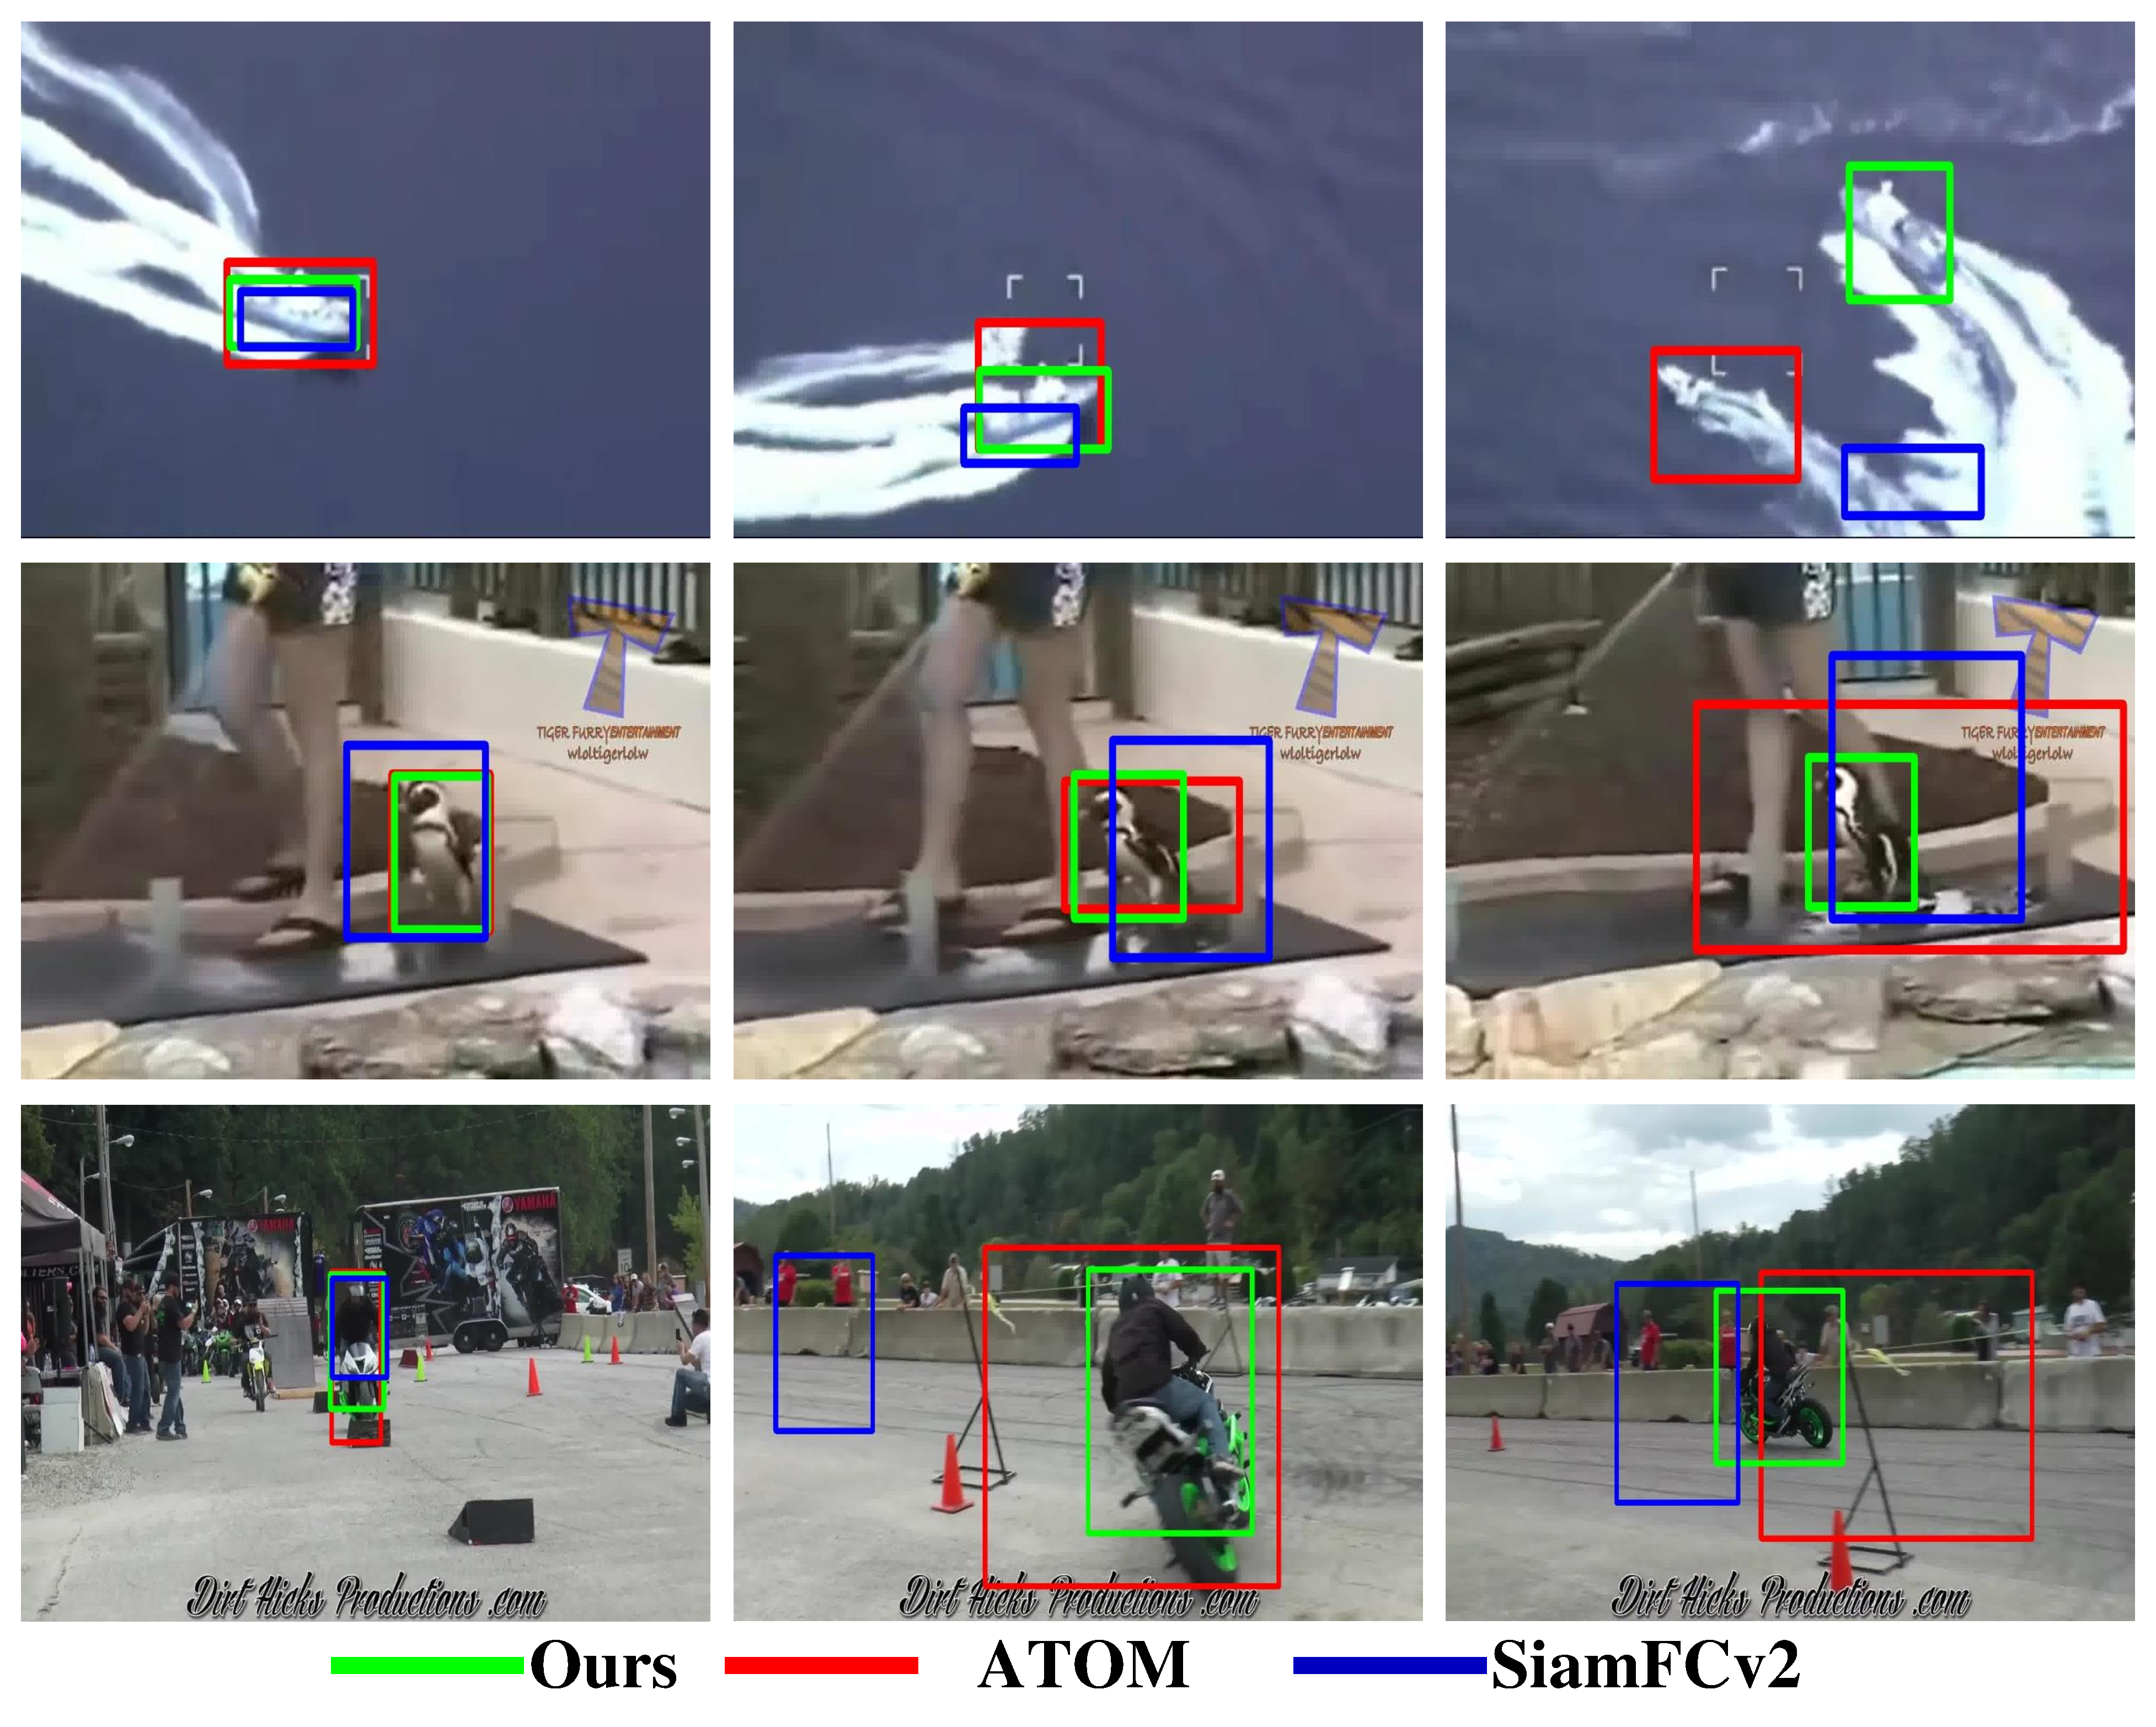
\includegraphics[width=0.48\textwidth]{images/got10k/visulization.pdf}
    \caption{AO of GOT-10k.}
\end{figure}

\IEEEPARstart{O}{beject} tracking is the task of getting target position and bounding box in every frame, giving the first frame annotation. Model updating is always an important part in object tracking. Because we need to know the information of the current video. DCF trackers can do it well, it use the first frame to train a ridge regression. However, the backbone is trained in ImageNet, so the performance is over by new tracking system--siamese trackers. 
[copy from Learning the Model Update for Siamese Trackers: start]
The basic principle of these trackers is to match an object appearance template with a corresponding feature representation of the search region in the test frame. The features for the object template and the search region are
acquired through a deep neural network trained offline on a large dataset.
In the original Siamese tracker [1], the object template is initialized in the first frame and then kept fixed during the remainder of the video. However, appearance changes are often large and failing to update the template could lead to early failure of the tracker. In such scenarios, it is important to adapt the model to the current target appearance.
[copy from Learning the Model Update for Siamese Trackers: end]
It offline learn embedding network. During tracking, the model is fixed. Due to the new architecture and large training dataset, it's performance is good. Recently, researchers find that the drawback of Siamese networks is that it cannot online upgrade. So many researchers try to use current video information in Siamese tracker. They can be categories into 2 ways: model update and template update. For model update, they want to change the parameters using the first frame. However, it may destroy the offline learned parameters, break the generalization ability, easy cause overfitting. The next method is template update, combine the template at the history frames. However, template update only focus on the appearance change, they do not use the first ground truth. What's more, it's hard to select the most confident template, once use the wrong template, will cause accumulate error.

To find a better way to model update using the first frame, instead of modify the model parameter, we find a new way to achieve this: according to the adversarial example thought with some change, we change the template with small change, to make the prediction better.
Specifically, given the input image, the siamese network input compose of two parts: search image and template image. At the first frame, we are given the ground truth bounding box. we use the popular adversarial example generation method. Specifically, we use the ground truth to calculate the loss. Then we calculate the gradient with respect to the template.
Then we use the gradient to update the template, so the loss is smaller. We continue this loop until a fixed number.
At the following tracking process, we use the new kernel. By doing so, we can utility the current frame information, and still protect the offline learned siamese network parameter.
Our model is pluggable, do not need to change the network, and fast, with 82 FPS.
By change the input, we achieve the state-of-the-art performance on 4 challenging tracking dataset.

\section{Proposed Algorithm} 
[copy from Learning the Model Update for Siamese Trackers: start]
In this section, we present our approach to learn how to update the object template during online tracking. We start
by revisiting the standard update mechanism in tracking and identifying its drawbacks. Then, we introduce our formulation to overcome them and describe our model and training procedure in detail. The focus of this paper is on Siamese
trackers. Note, however, that our approach is not limited to Siamese trackers and the same formulation could be applied
to other types of trackers, e.g. DCF [19, 11, 7].
[copy from Learning the Model Update for Siamese Trackers: end]

We formulate object tracking as a confidence-based regression problem: give output-input pair $(y,x)$, learns a function $s_\theta:\mathcal{Y\times X\rightarrow \mathbb R}$, and predict a scalar confidence score $s_\theta(y,x)\rightarrow\mathbb R$. The final estimate $f(x)=y^*$ is predicted as follows:
\begin{equation}
f(x) = \arg\max_{y\in \mathcal Y}s_\theta (y,x)
\end{equation}
The input $\mathcal X$ means the image space. $y$ indicates the regression objective, it could be the spatial position, or the entire target box. The optimization is:
\begin{equation}
L(\theta;x_i,y_i)=\int_{\mathcal Y}\ell(s_\theta(y,x_i),a(y,y_i))\ \mathrm{d}x
\end{equation}

Popular trackers are usually categorised into two aspect: (1) DCF trackers. (2) Siamese trackers.

The DCF tracker:
\begin{equation}
s_\theta(y,x)=(w_\theta * \phi(x))(y)
\end{equation}
where $w_\theta$ is the kernel, $\phi(x)$ is the image feature. The loss of DCF is $\ell(s,a)=(s-a)^2$. Pseudo labels of most DCF trackers are $a(y,y_i)=e^{-\frac{||y-y_i||^2}{2\sigma^2}}$.

Siamese trackers:
\begin{equation}
s_\theta(y,x)=(\phi_\theta(z) * \phi(x))(y)
\end{equation}
[copy from Learning the Model Update for Siamese Trackers: start]
It is a two-stream architecture. One stream extracts the object template’s features based on an exemplar image that contains the object to be tracked. The other stream receives as input a large search region in the target image. The two outputs are cross-correlated to generate a response map of the search region.
[copy from Learning the Model Update for Siamese Trackers: end]

They both have advantages and disadvantages: DCF only use the first frame to learn the model parameter $w$. The advantage is make full use of the appearance information of the current video. The disadvantage is: only rely on the information of the current information. The network $\phi$ is trained at ImageNet dataset, which is not good for tracking task. It usually cannot use the large scale object tracking dataset for training such as GOT-10k.
For Siamese trackers, the advantage is use big data to offline train the network $\phi$. The disadvantage is can not use the information of the current video.
Our method combine both advantages of DCF trackers and Siamese trackers: Use siamese backbone, not changing network parameters during tracking, to preserve the offline learned information using big data, such as GOT-10k. On the other hand, we want to do model adaptation like DCF.

But how can we achieve this goal ? By analyse the DCF and Siamese formulation. We found they have common aspect:

The traditional siamese trackers update $\phi_\theta$. We think it is a bad idea because it may destroy the offline learned features. However we update $z$.

Compare the above formulations, no matter what is the detailed architecture, we just simply represent them as $\phi$, we can see the only difference is the update term, i.e., kernel, is different. DCF focus on $w$ using the current video information, while the $\phi(x)$ remains fixed. For Siamese trackers, they learn a good $\phi$ using large scale dataset, but can not use the current video information, thus no model update.

Based on the above observation, we propose a new method, using the common aspect of DCF/Siamese trackers, takes both advantages.

We can see that the $\phi_\theta(z)$ is equal to the $w_\theta$, we want to change $\phi_\theta(z)$, but we do not want to change $\phi$, so our solution is: change $z$. This solution is first proposed in this paper. We name it as model adaptation. Different from tradition model adaptation, they focus on changing the model parameters using the first frame. Different from traditional template update, they use hand crafted method to update template in every K frames. They do not change anything at the first frame, only use the history information to capture new appearance. Our method use the first frame ground truth, but not change the model parameters, but change the template image, so we call it template adaptation.

By doing so, the network can fix the offline learning ability, (other adaption method break this) at the same time doing model adaption like DCF. 

Now the problem is how to update $z$.

\subsection{Update z by inverse use adversarial example thought}

\begin{table}
\caption{The compare between our method and other methods}
\small
\setlength{\tabcolsep}{3pt}
\begin{tabular}{l c c c}
\toprule
                                 & Model update & Template update & Ours \\
\midrule
Modify model parameters          & Yes          & No              & No   \\
Use the first frame GT           & Yes          & No              & Yes  \\
Modify the template              & No           & Yes             & Yes  \\
\bottomrule
\end{tabular}
\end{table}

At the first glace, there is no connection between model adaptation and adversarial example. Because the purpose is different. The traditional adversarial example is used to make the model predict wrong result, making little change on the input image. However, our purpose is to make the model predict good result, making little change on the input template image. At the following, we will point out they have common aspect and only use the little change, we can utility the state-of-the-art adversarial example generation method to do template update. Before introduce our template update method, we first introduce the popular adversarial example generation method: 

Basic Iterative Method \cite{kurakin2017adversarial}: 

\begin{equation}
\begin{gathered}
    x_0^{adv} = \pmb X, \\
    x_{N+1}^{adv} = Clip_{X,\epsilon}\{\pmb X_N^{adv}+\alpha \text{ sign}(\nabla_X L(\pmb X_N^{adv},y_{true}))\}
\end{gathered}
\end{equation}

Iterative Target Class Method
\begin{equation}
\begin{gathered}
x_0^{adv} = \pmb X,\\
x_{N+1}^{adv} = Clip_{X,\epsilon}\{\pmb X_N^{adv}-\alpha \text{ sign}(\nabla_X L(\pmb X_N^{adv},y_{target}))\}
\end{gathered}
\end{equation}

We can see that, the adversarial example can work well, is because they use wrong label to calculate gradient, and modify the input to make the network predict to the wrong label. It is really fast and works very well.

But what is the connection between adversarial examples and the template update ? The answer is, we also modify the template image, but we use the True label, not the wrong label:

\begin{equation}
z_0 = z, z_{N+1} = Clip_{z,\epsilon}\{z_N -\alpha \text{ sign}(\nabla_z L(z_N,y_{true}))\}
\end{equation}
where $L$ means the loss function.

Note that the first frame label is always given at the tracking task, which makes the above equation make sense. By doing so, the prediction is better at the first frame. At this process, we modify the appearance of the template, which introduce the per-video information and can tracking good at following frames. Note that only the first frame label is given, so we only do template update at the first frame, make sure the correctness.

\begin{figure}[t]
    \centering
    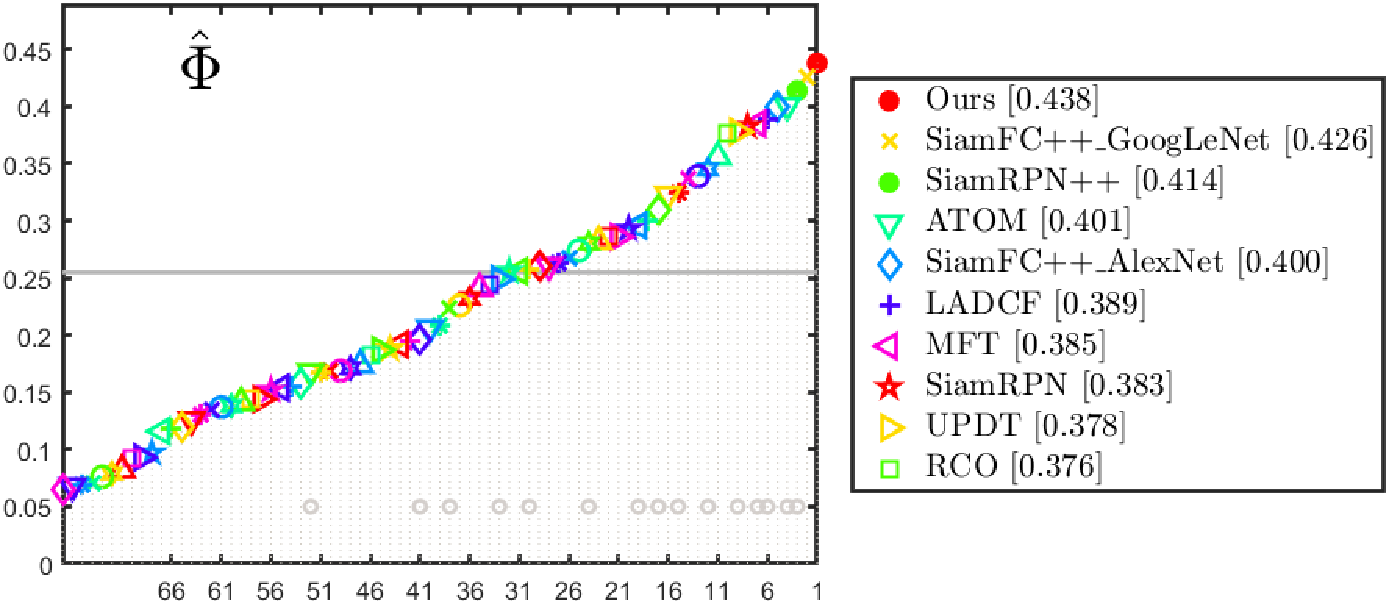
\includegraphics[width=0.48\textwidth]{images/vot18/vot18_eao.pdf}
    \caption{EAO of VOT2018.}
\end{figure}

Recently, some work focus on model update.
However, all of them perform on the weights, which has so many parameters, all of them need to be updated, which easily cause overfitting and computation cost. To solve these problems, many method design complex strategy to escape from overfitting and lower the computation.
However, is there a simpler toolkit for solving these tasks ? [4]
However, we only need to update the input tensor of shape $3\times 128\times128$. The benefits are two folders:
(1) escape from overfitting.
(2) speed up.
To solve this problem, many researches [16, 45, 40] present different mechanisms to update template features. However, these methods only focus on combining the previous target features, ignoring the discriminative information in background clutter. This results in a big accuracy gap between the siamese-based trackers and those with online update. [1]

We are the  first to update the template.

Generally, adversarial examples is used to attack the network. However, we use it to update the template.

At a high level, our adaptation procedure is based on minimizing the loss of a tracker. [4]

We propose the adversarial update tracker (AUTracker), with adversarial module, to online update as shown in Fig. 2. AUTracker is built upon the siamfc++ tracker, with a target classification branch and a target localization branch. The classification branch converts the feature map into a response map and provides the coarse locations of the target. The localization branch uses the bounding-box regression to localize targets. the adversarial module is applied in a plug-and-play manner, as shown in Fig. 3. [2]

We introduce a adversarial module for online update that is pluggable, in the sense that it does not alter the overall architecture of the base tracker.

The module takes as input the target $z$ and search region $x$ in the first frame, and outputs a new input $z'$.

The follow-up tracking procedure remains unchanged.

The template generation process consists of initial embedding, gradient calculation and template updating.

1. First, the template image $z\in\mathbb R^{3\times128\times 128}$ is send to the siamese backbone $\phi$ to obtain an initial template $\beta$ which is used to calculate the initial loss L.
2. Second, the gradient of the whole tracker is calculated through backward propagation.
3. Finally, the gradient of the template image is subtracted to template image to get an updated target image. [1]

\begin{table}
\centering
\caption{Comparing the results of our approach against other approaches over the Tracking Net.}
\begin{tabular}{l c c c}
\toprule
Method   &  Prec.   &  Norm. Prec. & Succ  \\
\midrule
Ours  &  70.6&  81.7 &74.9 \\
SiamFC++ GoogLeNet& 70.5 & 80.0 & 75.4 \\
SiamFC++ AlexNet  & 64.6 & 75.8 & 71.2 \\
ATOM              & 64.8 & 77.1 & 70.3 \\
SiamRPN++&  69.4 & 80.0 &73.3 \\
MDNet	 &  56.5&  70.5 &60.6 \\
ECO	 &  49.2&  61.8 &55.4 \\
SiamFC	 &  51.8&  65.2 &55.9 \\
\bottomrule
\end{tabular}
\end{table}

\subsection{Tracking framework with template adaptation}
We describe how the template adaption is applied for online tracking.
The input the network compose of search image and template image.
They share same feature extractor.
For the initial step, the search image is the first frame image, the template image is the image patch cropped from the first image according to the ground truth bounding box.
We get the tracking prediction using these two inputs: classification prediction and regression prediction.
Because we have the ground truth, so we can calculate the Loss:

\begin{equation}
\begin{split}
L(\{p_{x,y}\},q_{x,y},\{\pmb t_{x,y}\}) &= \frac{1}{N_{\text{pos}}}\sum_{x,y}L_{\text{cls}}(p_{x,y},c^*_{x,y})\\
&+\frac{\lambda}{N_{\text{pos}}}\sum_{x,y}\pmb1_{\{c^*_{x,y}>0\}}L_{\text{quality}}(q_{x,y},q^*_{{x,y}})\\
&+\frac{\lambda}{N_{\text{pos}}}\sum_{x,y}\pmb1_{\{c^*_{x,y}>0\}}L_{\text{reg}}(\pmb t_{x,y},\pmb t^*_{{x,y}})
\end{split}
\end{equation}

Where $L_{\text{cls}}$ is the focal loss. $L_{\text{quality}}$ is the binary cross entropy (BCE) loss for quality assessment. $L_{reg}$ is the IoU loss for bounding box regression.

$\pmb t^*=(l^*,t^*,r^*,b^*)$. The regression target at position $(x,y)$ is: 

\begin{equation}
\begin{split}
l^*=(\lfloor\frac{s}{2}\rfloor+xs)-x_0,\   &t^*=(\lfloor\frac{s}{2}\rfloor+ys)-y_0\\
r^*=x_1-(\lfloor\frac{s}{2}\rfloor+xs),\   &b^*=y_1-(\lfloor\frac{s}{2}\rfloor+ys)
\end{split}
\end{equation}

Use Prior Spatial Score (PSS) for quality assessment:
\begin{equation}
\text{PSS}^* = \sqrt{\frac{\min(l^*,r^*)}{\max(l^*,r^*)}\times\frac{\min(t^*,b^*)}{\min(t^*,b^*)}}
\end{equation}

Next we calculate the gradient with respect to the template z, and subtraction it with z to get new z.
Loop to a fixed step, so we get new template image z'.
For the following steps, the search image is next frame, and the template is z' instead of z.

We adopt SiamFC++ as the basic tracker. fx(.) is used to model the feature extraction branch for search region, fz(.) is used to model the feature extraction branch for target region. We assume that the movement of the target is smooth between two consecutive frames. Thus, we can crop a search region X which is larger than the target patch Z in the current frame, centered at the target’s position in the last frame. The final score map is calculated by: ...

Sepcifically, we adopt the Basic Iterative Method (BIM) to generate the new input.

We expect to obtain $z'$ from $z$, such that, after $N$ steps of pixel update on support set $(z, x_0)$ to obtain $z'$, the tracker performs well on query set $(z', x_i)$.

The $i$th gradient update step on $z'$ can be expressed as:
$$
z_0 = z, z_{N+1} = Clip_{z,\epsilon}\{z_N -\alpha \text{ sign}(\nabla_z L(z_N,y_{true}))\}
$$

The AU module is inspired by the AIM developed for adversarial training. However, AU is different from the adversarial training from the following two aspects: 1) AU targets at update the target appearance so that loss can be well fitted to make the prediction better. In contrast, the AIM modify inputs to make the prediction bad; 2) PRP leverages more efficient row- and column-wise maximization operations to aggregate the large response to target centers, while the center/corner pooling uses comparison and substitution operations. [2]

\iffalse
\begin{table}
\begin{center}

\begin{tabular}{c c|c c}
\toprule
\multicolumn{2}{c|}{Trackers} & 
\begin{tabular}{c} \textbf{SiamFC++-} \\ \textbf{GoogLeNet} \end{tabular} &
\begin{tabular}{c} \textbf{Ours} \\ \textbf{GoogLeNet} \end{tabular} \\

% OTB
\midrule
\multirow{1}{*}{OTB-15} 
& Success & 68.3 & 69.7\\
% VOT
\midrule
\multirow{3}{*}{VOT-18}
& A   & 0.587 & 0.591 \\
& R   & 0.183 & 0.187 \\
& EAO & 0.426 & 0.438 \\

% GOT-10k
\midrule
\multirow{3}{*}{GOT} 
& SR\textsubscript{.5} &  69.5 & 74.8 \\
& SR\textsubscript{.75} & 47.9 & 47.5 \\
& AO & 59.5 & 61.7 \\
% TrackingNet
\midrule
\multirow{3}{*}{T-Net} 
& Prec.       & 70.5 & 70.6 \\
& Norm. Prec. & 80.0 & 81.7 \\
& Succ.       & 75.4 & 74.9 \\
% FPS
\midrule
\multicolumn{2}{c|}{FPS} & 90 & 82\\
\bottomrule
\end{tabular}

\end{center}
\caption{Results on several benchmarks. T-Net denotes TrackingNet. Top-3 results of each dimension (row) are colored in red, green, and blue, respectively.}
\label{tab:benchmark results}
\end{table}
\fi

\section{Experiments}

In this section, we compare our method with different methods on four tracking dataset. 
Our baseline method is SiamFC++. We add our module on it. The performance improvement compared with the baseline method is provided at every dataset. We also provide the implementation detail and speed analysis at following.

\begin{figure}[t]
    \centering
    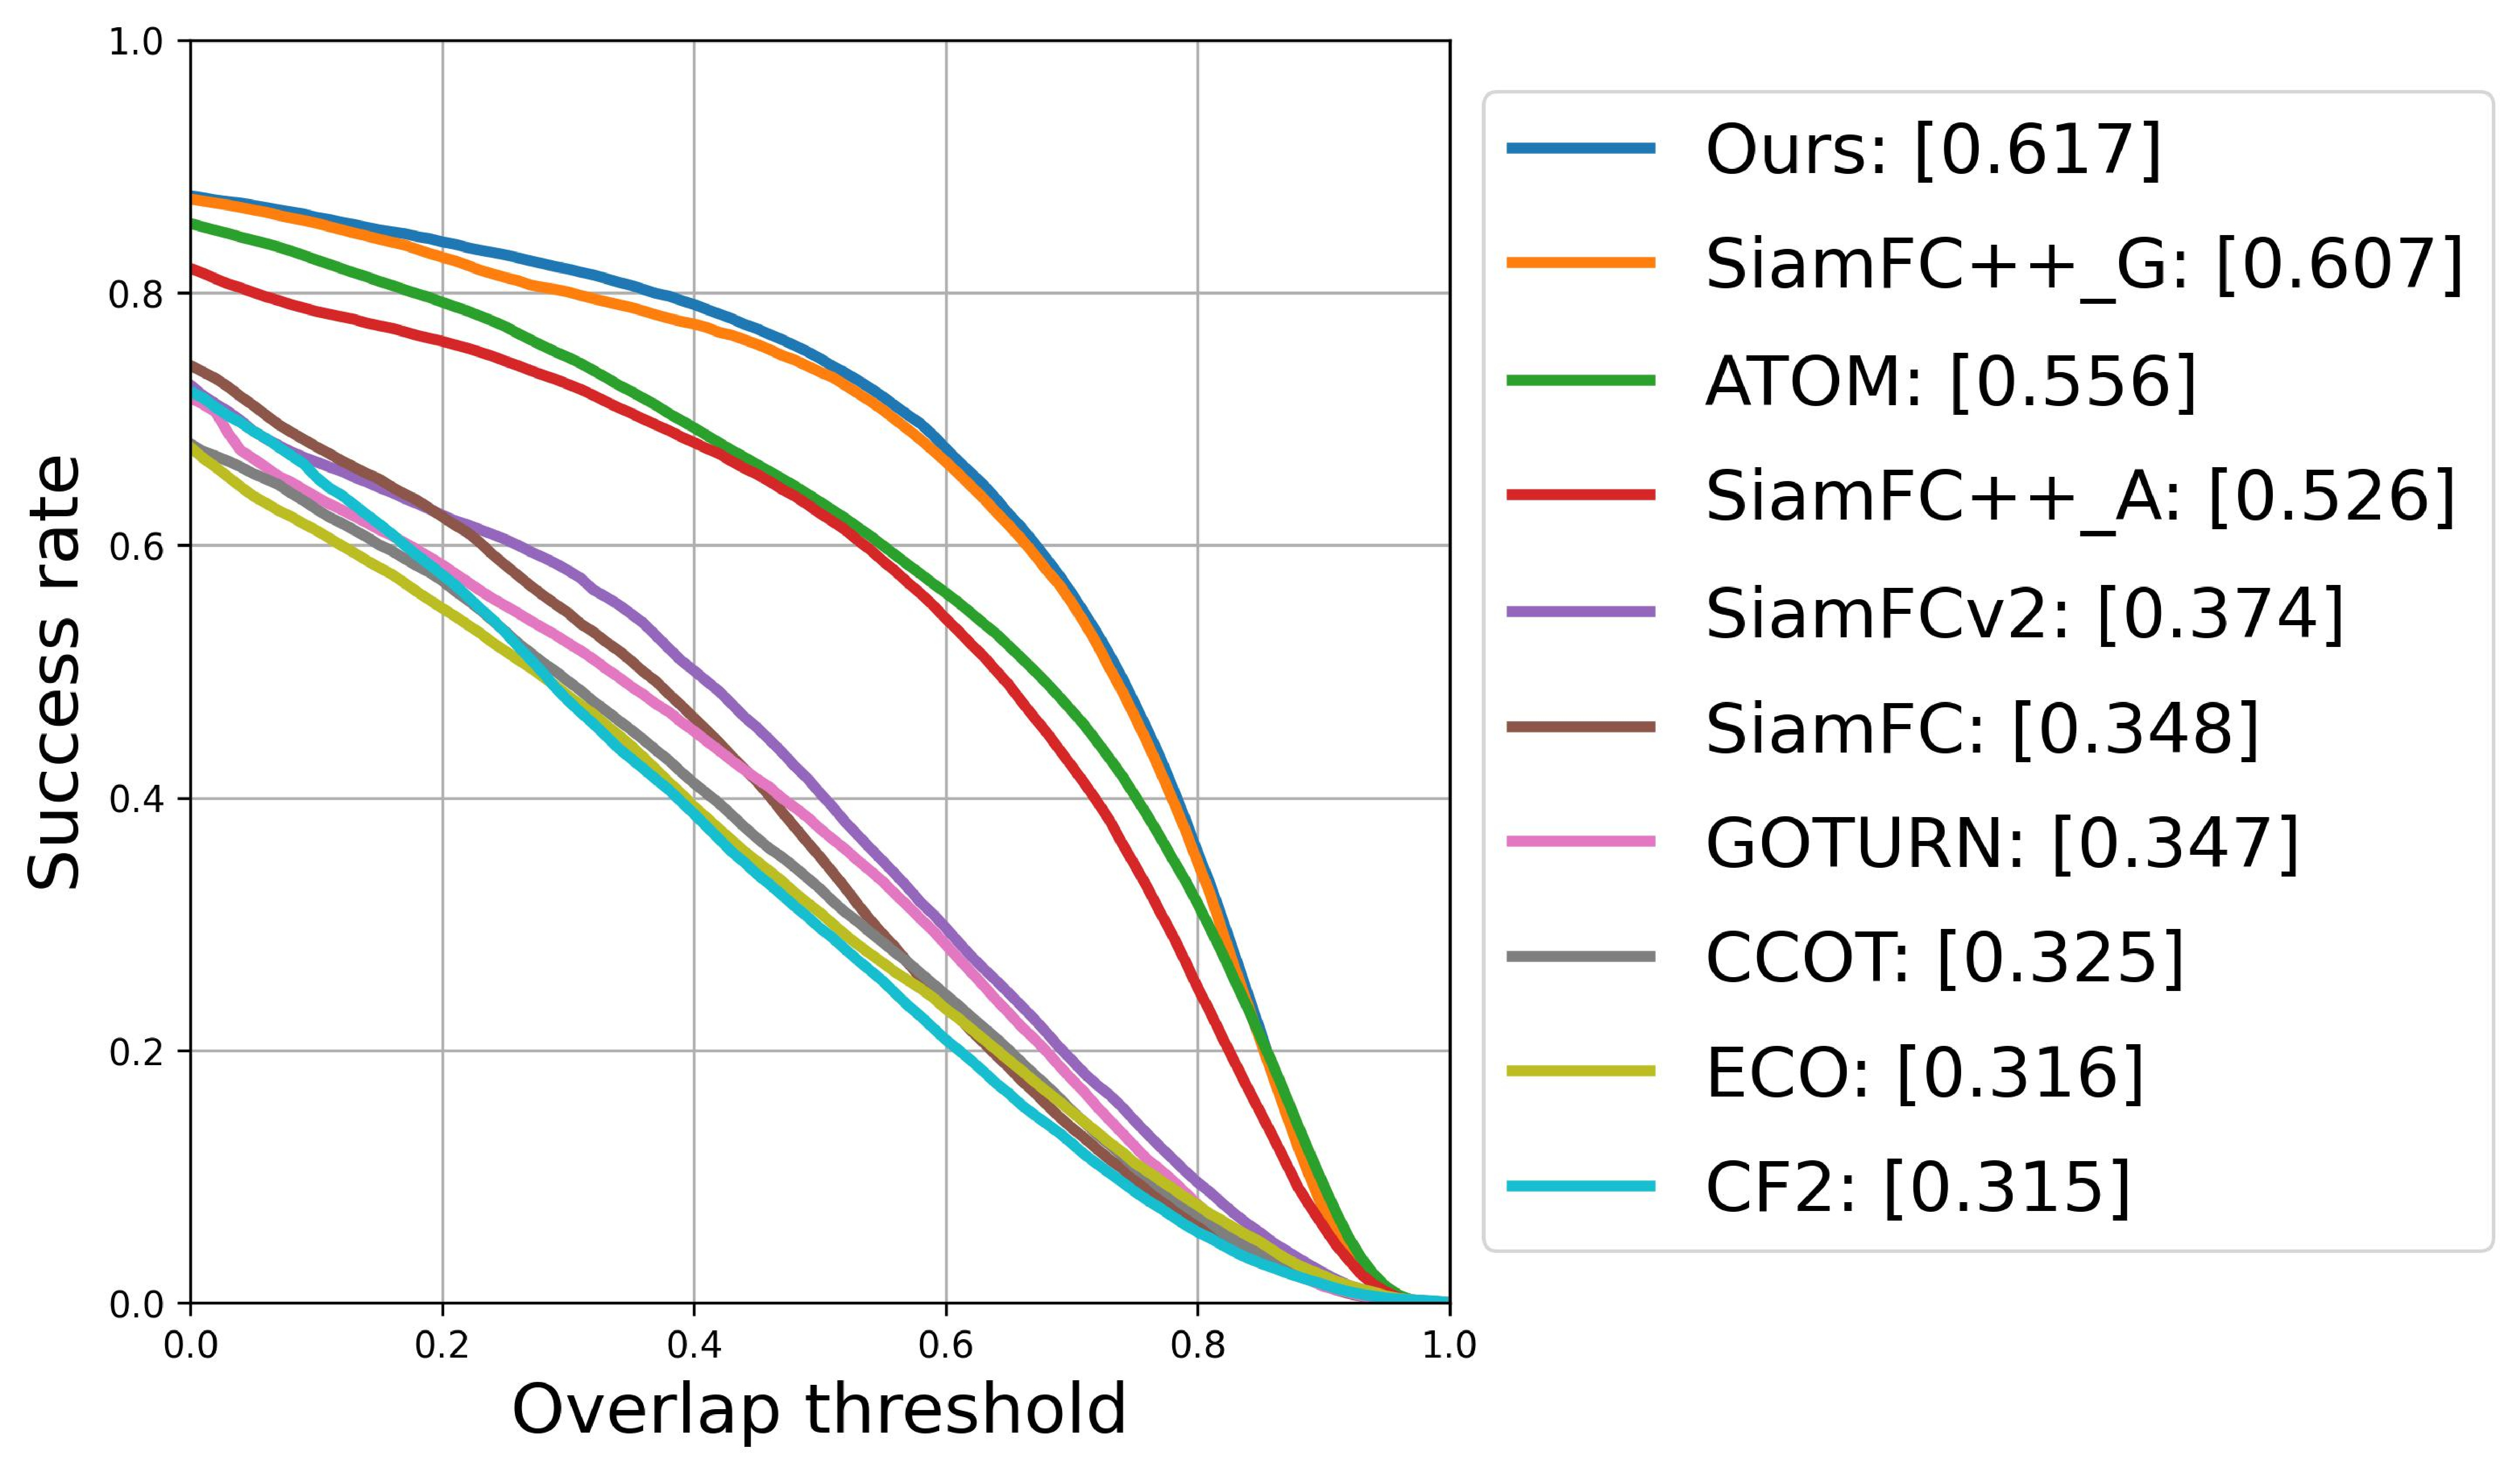
\includegraphics[width=0.4\textwidth]{images/got10k/got10k_ao.pdf}
    \caption{AO of GOT-10k.}
\end{figure}

\subsection{Implementation details}
We use SiamFC++ as the tracker. The description is introduced as following:
It is a Fully Convolutional Siamese tracker++ (SiamFC++) by introducing both classification and target state estimation branch (G1), classification score without ambiguity (G2), tracking without prior knowledge (G3), and estimation quality score (G4).
For detailed information, please refer to [...].
The template size is 127*127, the search size is 289*289.
We do not train the network. Which is very good.

\subsection{Results on VOT Benchmark}
[copy from SiamFC++: start]
VOT2018 contains 60 video sequences with several challenging topics including fast motion, occlusion, etc. We test our tracker on this benchmark and present the results in Table .... Both versions of our trackers reaching comparable scores w.r.t. current state-of-the-art trackers, the tracker with AlexNet backbone outperforms other trackers with the same tracking speed and while the tracker with GoogLeNet backbone yields a comparable score. Besides, our tracker has a significant advantage in the robustness among the trackers in comparison. To the best of our knowledge, this is the first tracker that achieves an EAO of 0.400 on VOT2018 benchmark while running at a speed over 100 FPS, which demonstrate its potential of being applied in real production cases.

\begin{table}[t]
\caption{Result on OTB15.}
\setlength{\tabcolsep}{3pt}
\begin{center}
\begin{tabular}{l | c c c c c c}
\toprule
Trackers & ECO  & MDNet & SiamRPN++ & ATOM & SiamFC++\_G & Ours \\
\midrule
Success & 70.0 & 67.8  & 69.6      & 66.9      & 68.3       & 69.7 \\
FPS     & 8    & 1     & 35        & 30       & 90         & 82  \\
\bottomrule
\end{tabular}
\end{center}
\end{table}

\subsection{Results on LaSOT Benchmark}
With a large number of video sequences (1400 sequences under Protocol I while 280 under Protocol II), LaSOT~\cite{fan2019lasot} (Large-scale Single Object Tracking) benchmark makes it impossible for trackers to overfit the benchmark, which achieves the purpose of testing the real performance of object tracking. Following Protocol II under which trackers are trained on LaSOT \textit{train} subset and evaluated on LaSOT \textit{test} subset, the proposed SiamFC++ tracker achieves better performance, even w.r.t. those who have better performance than ours on the VOT2018 benchmark. This reveals the fact that the scale of the benchmark influences the rank of trackers. 

\subsection{Results on GOT-10k Benchmark}
For target class generalization testing, we train and test our SiamFC++ model on GOT-10k~\cite{huang2018got} (Generic Object Tracking-10k) benchmark. Not only as a large-scale dataset (10,000 videos in train subset and 180 in both \textit{val} and \textit{test} subset), it also gives challenges in terms of the requirement of category-agnostic for generic object trackers as there is no class intersection between \textit{train} and \textit{test} subsets. We follow the protocol of GOT-10k and only trained our tracker on the \textit{train} subset. Our tracker with AlexNet backbone reaches an AO of 53.5 surpassing SiamRPN++ by 1.7, while our tracker with GoogLeNet backbone yields 59.5 which is even superior to ATOM that uses online updating method. This result shows the ability of our tracker to generalize even the target classes are unseen during the training phase, which matches the demand of the generic tracking.

\subsection{Results on TrackingNet Benchmark}
We evaluate our approach with 511 videos provided in the \textit{test} split of TrackingNet~\cite{muller2018trackingnet}. We exclude the Youtube-BB dataset from our training data in order to avoid data leak. As is described in \cite{muller2018trackingnet}, the evaluation server calculates the following three indexes based on tracking results: success rate, precision, and normalized precision. Our SiamFC++-GoogLeNet outperforms the current state-of-the-art methods (including online-update methods like \cite{danelljan2019atom}) in both precision and success rate dimensions, while our lightweight version SiamFC++ strikes a balance between performance and the speed. This result is achieved even without Youtube-BB containing a large portion of training data, which shows that the potential of our approach to be independent of large offline training data.
[Copy from SiamFC++: end]

\section{Conclusion}

A conclusion section is not required. Although a conclusion may review the main points of the paper, do not replicate the abstract as the conclusion. A conclusion might elaborate on the importance of the work or suggest applications and extensions. 

\newpage
\bibliographystyle{IEEEbib}
\bibliography{refs}


\end{document}